% This is samplepaper.tex, a sample chapter demonstrating the
% LLNCS macro package for Springer Computer Science proceedings;
% Version 2.21 of 2022/01/12
%
\documentclass[runningheads]{llncs}
%
\usepackage[T1]{fontenc}
% T1 fonts will be used to generate the final print and online PDFs,
% so please use T1 fonts in your manuscript whenever possible.
% Other font encondings may result in incorrect characters.
%
\usepackage{graphicx}

\usepackage{loadpkg_lncs}
\usepackage{makecell}
\graphicspath{{./images/}}
\setlength\tabcolsep{7pt}
% Used for displaying a sample figure. If possible, figure files should
% be included in EPS format.
%
% If you use the hyperref package, please uncomment the following two lines
% to display URLs in blue roman font according to Springer's eBook style:
%\usepackage{color}
%\renewcommand\UrlFont{\color{blue}\rmfamily}
%\urlstyle{rm}
%
\begin{document}
%
\title{Deep learning approaches for Video-based Gym Exercise Classification}
%
%\titlerunning{Abbreviated paper title}
% If the paper title is too long for the running head, you can set
% an abbreviated paper title here
%
\author{Xuan-Cuong Nguyen,\inst{1}\orcidID{0000-1111-2222-3333} \and
Nhat-Quang Truong\inst{2,3}\orcidID{1111-2222-3333-4444} \and
Third Author\inst{3}\orcidID{2222--3333-4444-5555}}
%
\authorrunning{X.-C. Nguyen et al.}
% First names are abbreviated in the running head.
% If there are more than two authors, 'et al.' is used.
%
\institute{FPT University - Da Nang Campus, Da Nang 550000, Viet Nam
\email{cuongnxde180528@fpt.edu.vn}\\
% \url{http://www.springer.com/gp/computer-science/lncs} \and
% ABC Institute, Rupert-Karls-University Heidelberg, Heidelberg, Germany\\
% \email{\{abc,lncs\}@uni-heidelberg.de}
}
%
\maketitle              % typeset the header of the contribution
%
\begin{abstract}
Gym exercises have played an important role in modern life as they can help improve both physical fitness and mental health for people.
For a modern busy lifestyle, people often intend to do gym workouts at home instead of in fitness centers.
Consequently, it is necessary to build a virtual personal trainer to help busy people mitigate injury risks and optimize outcomes when doing gym workouts at home.
A fundamental component of this system is to recognize the exercises in real-time.
Raw gym videos are first manually trimmed into clean segments and sampled into fixed‐length clips for downstream processing. We propose a framework that captures both skeletal and graph‐based representations: a pose stream in which MediaPipe detects 33 key 3D landmarks per frame—each re‐centered on the nose and converted into relative coordinates and joint angles computed via triplet permutations—and modeled with temporal models including LSTM, Bi-LSTM, and a lightweight Transformer encoder; and a graph stream that constructs a spatio‐temporal joint graph from the same landmarks and processes it through an ST‐GCN to directly learn dynamic relationships among connected joints. We evaluate our approach on a self‐collected dataset of 1\,026 clean videos covering 22 common gym exercises. Experimental results demonstrate that fusing relative landmark‐based features, joint angles, and graph‐convolutional modeling with stacking ensembling yields 66.19\% classification accuracy on the test set, underscoring the importance of combining relative skeletal cues and structured joint dynamics for accurate, real‐time exercise recognition.
\keywords{Gym exercise classification \and pose estimation \and MediaPipe \and ST-GCN \and LSTM \and Transformer \and feature engineering \and temporal modeling \and human action recognition.}
\end{abstract}
%
%
%
\section{Introduction}

As general living standards rise, more individuals turn to gym workouts to bolster both physical fitness and mental well–being. 
Yet without expert supervision, home exercisers often adopt incorrect form, risking injury or suboptimal results. 
A virtual personal trainer must first recognize which exercise is being performed; only then can it deliver timely feedback and correction. 
Recent advances in deep learning—especially video transformers—make it possible to tackle this recognition task with high accuracy directly from raw footage.

In this study, a two-branch framework for gym exercise classification is introduced. 
The pose branch leverages MediaPipe to extract 33 key 3D landmarks per frame—each re-centered on the nose and converted into relative coordinates and joint angles computed via triplet permutations—and models these feature sequences with a compact Transformer encoder. 
The graph branch constructs a spatio-temporal joint graph from the same landmarks and processes it through an ST-GCN to directly capture dynamic relationships between body joints. 
Experiments on a self-collected dataset of 1024 clean clips spanning 22 gym exercises demonstrate that fusing landmark-based and graph-based representations significantly outperforms either branch alone, highlighting the benefit of combining relative skeletal features with explicit joint-graph modeling for accurate, real-time exercise recognition.

\section{Related Work}

To classify the actions using videos, many methods have been proposed. In this section, the literature review of these methods is presented.

In 2015, Donahue et al. introduced a CNN-LSTM framework for action classification that integrated convolutional neural networks for spatial feature extraction with LSTM networks for temporal modeling. 
Their model, evaluated on datasets such as UCF101, reported a top-1 accuracy of approximately 82\% \cite{donahue2015}. 
Although this hybrid approach successfully captured both appearance and motion cues, it was hindered by high computational complexity and challenging training dynamics due to the integration of convolutional and recurrent components.

Building upon early CNN-LSTM methods, landmark-based LSTM approaches emerged around 2016. 
For instance, Li et al. (2016) proposed a method where skeletal keypoints are extracted via pose estimation and then fed into an LSTM network for action recognition. 
Evaluated on the NTU RGB+D dataset, their approach achieved roughly 86\% accuracy on the cross-subject protocol \cite{li2017}. 
This method benefits from a reduced computational load by focusing on essential body movements rather than full images; however, its performance is highly dependent on the quality of the underlying pose estimation, with inaccuracies in landmark extraction significantly affecting the final results.

In 2018, Yan et al. advanced the field with the introduction of the Spatial Temporal Graph Convolutional Network (ST-GCN), which models the human skeleton as a graph where keypoints serve as nodes and anatomical connections as edges. 
Tested on the NTU RGB+D dataset, ST-GCN obtained 81.5\% accuracy under the cross-subject setting and up to 88.3\% in the cross-view configuration \cite{yan2018}. 
The strength of ST-GCN lies in its simultaneous modeling of spatial configurations and temporal dynamics; nevertheless, its reliance on accurate skeleton extraction and predefined graph structures limits its robustness, especially in the presence of noisy or incomplete data.

More recently, the adoption of transformer-based architectures has led to further improvements in action classification. 
Arnab et al. extended the Vision Transformer (ViT) paradigm to the video domain with the ViViT model, which applies self-attention mechanisms over image patches to capture long-range dependencies across frames \cite{arnab2021}. 
Evaluated on the Kinetics-400 dataset, ViViT achieved a top-1 accuracy of approximately 77\% . Although transformer-based models excel at capturing global context, they require extensive training data and significant computational resources, which can be a critical limitation for practical deployment.

In 2024, Nguyen et al. extended landmark-based LSTM methods to exercise classification on a four-class dataset (barbell biceps curl, push-up, squat, shoulder press) by extracting 22 body keypoints and 12 joint-angle features per frame and feeding them into a bidirectional LSTM. 
Evaluated on 791 test windows, their BiLSTM model achieved near-perfect performance—overall accuracy of 0.99, with F1-scores of 0.99 for curl, 1.00 for push-up, 0.98 for squat, and 1.00 for shoulder press . 
They generated overlapping 30-frame windows from each video and then randomly shuffled all windows before splitting into train/validation/test sets at a 70\%–15\%–15\% ratio . 
While this approach yields impressive metrics, it permits windows from the same video to appear across different splits—introducing data leakage that inflates test performance—and relies on a fixed window length that may not generalize well to varying movement speeds or durations.  \cite{riccio2024}

Overall, these studies reflect a progressive evolution in action recognition. Early methods such as CNN-LSTM and landmark-based LSTM provide effective spatial-temporal integration, yet they face challenges related to computational cost and sensitivity to input quality, respectively. 
In contrast, ST-GCN leverages the structural information of the human skeleton but depends on high-quality pose data, while transformer-based approaches like ViViT offer superior global context modeling at the expense of increased data and computational requirements. 
These varied outcomes underscore the importance of developing robust systems that blend the complementary strengths of these techniques for efficient and accurate action classification.

\section{Dataset}


\begin{figure}[!h]
    % \hspace*{-1.5cm} % <-- Đẩy ảnh qua bên trái
    \begin{center}
    \resizebox{0.9\textwidth}{!}{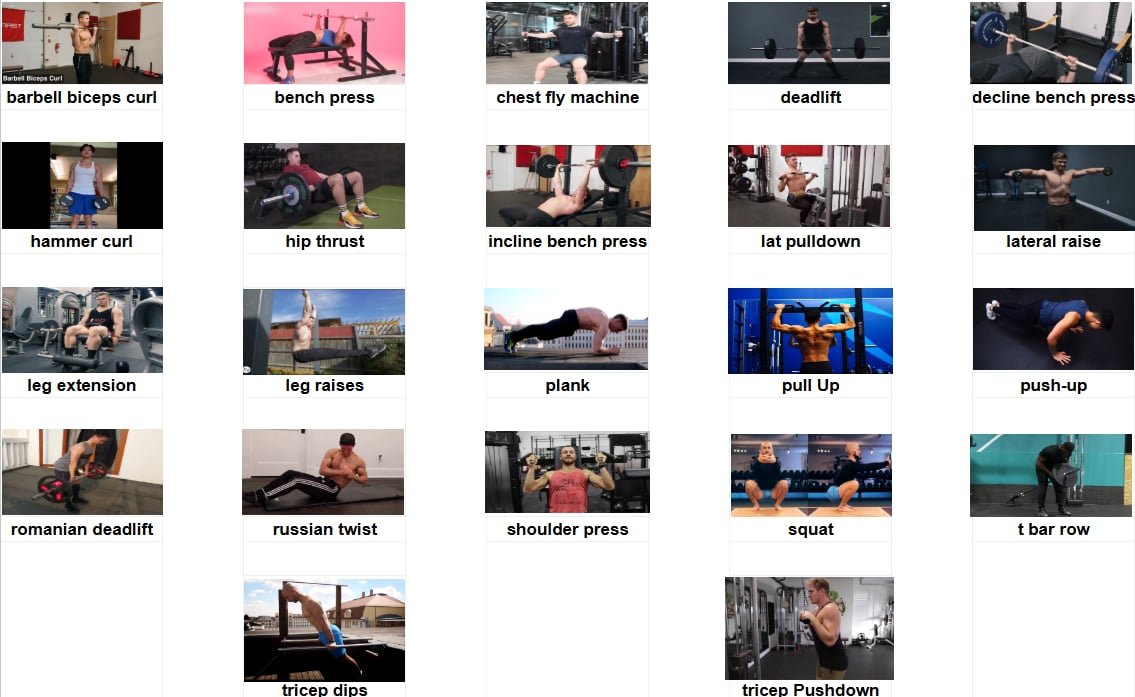
\includegraphics{./images/Dataset.png}}
    % \begin{tikzpicture}[
% Control the style of the blocks
%     node distance=1cm and 0.8cm,
%     base/.style={draw, fill=blue!20, text centered, minimum height=3em, rounded corners=3pt, font=\sffamily\small},
%     block/.style={base, text width=7em},
%     wideblock/.style={base, text width=9em},
    block/.style={
        draw,
        line width=0.3mm,
%         fill=red!10,
        minimum width=2.5cm,   % Your original width (1 - 0)
        minimum height=2cm,  % Your original height (1.5 - -2.5)
        align=center,
        font = \Large,
%         rotate=-90           % This rotates the whole box and text
    },
        blockfe/.style={
        draw,
        line width=0.3mm,
        fill=red!10,
        minimum width=3cm,   % Your original width (1 - 0)
        minimum height=4cm,  % Your original height (1.5 - -2.5)
        align=center,
        font = \Large,
%         rotate=-90           % This rotates the whole box and text
    },
    dataset/.style={
        draw,
        line width=0.3mm,
        fill=green!10,
        minimum width=4cm,   % Your original width (1 - 0)
%         width = 1cm,
        minimum height=1cm,  % Your original height (1.5 - -2.5)
        align=center,
        font = \Large,
%         rotate=-90           % This rotates the whole box and text
    },
    database/.style={
        draw, 
        cylinder, 
        aspect=0.3, 
        shape border rotate=90, 
        line width=0.3mm,
        minimum width=6em, 
        minimum height=8em, 
        text centered, 
        align=center,
       font = \Large,
    },
    sum/.style={
        draw,
        line width=0.3mm,
        circle,
        minimum size=0.5cm, % Matches your 0.25 radius
        inner sep=0pt,      % Ensures the '+' is perfectly centered
%         font=\small
    },
   model/.style = {
   draw, 
   rectangle, 
    minimum width=3cm, 
    minimum height=2cm, 
    line width = 0.3mm,
    align=center,
     font = \Large,
   },
    line/.style={draw, -Stealth, thick}, % stealth , -latex
    arrow/.style={draw, -Stealth, thick}
]





% \draw [line] (10,0) -- (11,1.5)-- (14,1.5)-- (14.5,1.5);
% \draw [line] (10,-0.5) -- (11,1)-- (14,1)-- (14.5,1);
% \draw [line] (10,-1) -- (11,0.5)-- (14,0.5)-- (14.5,0.5);

% \draw [line] (10,0) -- (11,-1.5)-- (14,-1.5)-- (14.5,-1.5);
% \draw [line] (10,-0.5) -- (11,-2)-- (14,-2)-- (14.5,-2);
% \draw [line] (10,-1) -- (11,-2.5)-- (14,-2.5)-- (14.5,-2.5);

% Nodes
%     \node [block] (segment) {Segment};
    \node [database] (database) at (-1,-0.5) {Video \\ dataset};
    \node [dataset] (training) at (4.5,1) {Training set};
     \node [dataset] (validation) at (4.5,-0.5) {Validation set};
     \node [dataset] (testing) at (4.5,-2) {Testing set};
%     \node [block, right=of data] (preproc) {Pre-Processing};
%     \node [block, right=of preproc] (pose) {Pose Estimation};
%     \node [block, right=of pose] (landmarks) {Landmarks};

\draw [line] (0,-0.5) -- (1,-0.5)-- (1,1)-- (training);
\draw [line]  (1,-0.5)-- (2,-0.5)-- (validation);
\draw [line]  (1,-0.5)-- (1,-2)-- (testing);




  
%   \node [sum] (sum1) at (16.5,-0.5) {+};
%  \draw [arrow] (14.5,1) -- (sum1.west);
%   \draw [arrow] (14.5,-2) -- (sum1.west);
%   
%     \node [sum] (sum2) at (16.5,-2) {+};
%  \draw [arrow] (14.5,0.5) -- (sum2.west);
%   \draw [arrow] (14.5,-2.5) -- (sum2.west);
  
   \node [dataset] (trainingfm) at (13.5,1) {Training set \\ feature maps};
     \node [dataset] (validationfm) at (13.5,-0.5) {Validation set\\ feature maps};
     \node [dataset] (testingfm) at (13.5,-2) {Testing set\\ feature maps};
     
        
\draw [arrow] (training.east) -- (trainingfm);
\draw [line] (validation.east) -- (validationfm);
\draw [line] (testing.east)-- (testingfm);

     
     \node [blockfe, fill opacity=0.9, text opacity=1] (feature) at (9,-0.5) {Feature \\ Extraction};
    
%     \draw [arrow] (sum.east) -- (trainingfm);
%     \draw [arrow] (sum1.east) -- (validationfm);
%     \draw [arrow] (sum2.east) -- (testingfm);
    \node [block] (seg) at (1,5.75) {\Large Segment};
    \node [block] (preproc) at (4.5,5.75) {\Large Preprocessing};
     \node [block] (pose) at (8.5,5.75) {\Large Mediapie-based \\ \Large pose landmark \\ \Large estimation};
%      \node [block] (landm) at (8.5,-6) {Landmark \\ extraction};
      \node [block, fill=cyan!10, fill opacity=0.9, text opacity=1] (angle) at (12.5,7.25) {\Large Angle \\ \Large Extraction};
    \node [block, fill=yellow!10, fill opacity=0.9, text opacity=1] (rel) at (12.5,4.25) {\Large Relative \\ \Large Landmark \\ \Large Extraction};
%       \node [sum] (sum) at (14,-6) {+};
      
       \draw [arrow] (-1,5.75) -- (seg) ;
        \draw [arrow] (seg) -- (preproc) ;
     \draw [arrow] (preproc.east) -- (pose) ;
%        \draw [arrow] (pose.east) -- (landm) ;
       \draw [arrow] (pose) -- (10.75,5.75)  -- (10.75,7.25)-- (angle);
       \draw [arrow] (10.75,5.75)  -- (10.75,4.25)-- (rel);
    
   
%  \draw [arrow] (angle)--(14,-5) -- (sum.north);
%   \draw [arrow] (rel)--(14,-7) -- (sum.south);
%     \draw [arrow] (sum)--(15,-6) ;
    
    \draw[dashed, line width = 0.3mm, red](-0.75,3) rectangle(16,8.5);
    
    \draw[ cyan!10,  fill = cyan!10 , line width = 0.3mm](15,5.75) rectangle(15.5,7.5);
    \draw[  yellow!10, fill = yellow!10 , line width = 0.3mm](15,4) rectangle(15.5,5.75);
     \draw[ black , line width = 0.3mm](15,4) rectangle(15.5,7.5);
     \draw[dashed](15,5.75)--(15.5,5.75);
    
    \draw [arrow] (angle)  -- (15,7.25);
    \draw [arrow] (rel)  -- (15,4.25);
    \draw [arrow] (15.5,5.75)  -- (16.25,5.75);
    
    \draw[dashed](-0.75,3)--(7.5,1.5);
      \draw[dashed](16,3)--(10.5,1.5);

\node[align = center, red] at (4.75,9) {\Large proposed feature extraction method for each frame};
\node[align = center] at (14.75,9) {\Large feature map};
\node[align = center, rotate = -90] at (14.75,5.75) {\Large concatenate};
 \draw[arrow, dashed](15.25,8.75)--(15.25,7.75);
 
 \node[model] (model) at (18,-0.5) {LSTM/ \\ BiLSTM/ \\ Transformer};
 \draw[arrow] (trainingfm) --(18,1)-- (model);
  \draw[arrow] (validationfm) -- (model);
  
  \node[model, red] (bestm) at (13.5,-4.75) {Best models};
   \draw[arrow] (model) --(18,-4.75)-- (bestm);
   \draw[arrow] (testingfm) -- (bestm);
   
   \draw[line width = 0.5mm] (8.75,-4.75) ellipse (1.5cm and 0.75cm);
\node[align = center] at (8.75,-4.75) {\Large Evaluations};
 \draw[arrow] (bestm) --(10.25,-4.75);
 
 \node[align = center] at (16.75,1.25) {\Large training};
  \node[align = center] at (14.5,-3.25) {\Large testing};
 
\end{tikzpicture}
    \end{center}
    \caption{Frame samples from 22 classes of gym exercises}
    \label{fig:pipeline}
\end{figure}

Study focuses on the automatic classification of 22 gym exercises, including barbell biceps curl, bench press, chest fly machine, deadlift, decline bench press, hammer curl, hip thrust, incline bench press, lat pulldown, lateral raise, leg extension, leg raises, plank, pull-up, push-up, Romanian deadlift, Russian twist, shoulder press, squat, t-bar row, tricep dips and tricep pushdown.

Dataset comprises 652 videos from a public Workout/Exercise Video Dataset \cite{abdillah2023}, 107 clips downloaded from YouTube fitness channels and 128 author-recorded videos, 65 videos from Pexels Website \cite{Pexels}, 76 videos from Freepik Website \cite{Freepik} for a total of 1024 unique sources. 
The dataset is split at the video level in a 6:2:2 ratio with the explicit aim of preventing content overlap between the training, validation, and test sets.

Each of these 1,024 videos was manually reviewed and cut into “clean” segments containing only the target exercise. On average, each video yielded 1.09 segments, producing 1,108 total segments: 639 in the training set, 210 in validation and 259 in test. 
Manual segmentation was critical to remove irrelevant frames such as transitions, rest periods or off-camera motion.

\begin{table}[!h]
\centering
\caption{Video and segment counts per exercise class by split}
\label{tab:counts-per-class}
\begin{tabular}{l r r r | r r r}
\hline
\multirow{2}{*}{\textbf{Class}}   & \multicolumn{3}{c|}{\textbf{Videos}} & \multicolumn{3}{c}{\textbf{Segments}} \\
  & \textbf{Train} & \textbf{Val} & \textbf{Test} & \textbf{Train} & \textbf{Val} & \textbf{Test} \\
\hline
barbell biceps curl    & 52  & 18  & 15  & 52  & 18  & 15  \\
bench press            & 51  & 18  & 15  & 51  & 18  & 15  \\
chest fly machine      & 28  & 9   & 8   & 28  & 9   & 8   \\
deadlift               & 30  & 10  & 10  & 30  & 10  & 10  \\
decline bench press    & 18  & 5   & 9   & 18  & 5   & 9   \\
hammer curl            & 24  & 8   & 14  & 24  & 8   & 14  \\
hip thrust             & 14  & 6   & 9   & 14  & 6   & 9   \\
incline bench press    & 27  & 10  & 9   & 27  & 10  & 9   \\
lat pulldown           & 43  & 15  & 14  & 43  & 15  & 14  \\
lateral raise          & 24  & 8   & 15  & 24  & 8   & 15  \\
leg extension          & 22  & 9   & 13  & 22  & 9   & 13  \\
leg raises             & 15  & 6   & 11  & 15  & 6   & 11  \\
plank                  & 5   & 2   & 2   & 5   & 2   & 2   \\
pull Up                & 31  & 11  & 10  & 31  & 11  & 10  \\
push-up                & 40  & 14  & 12  & 40  & 14  & 12  \\
romanian deadlift      & 12  & 6   & 6   & 12  & 6   & 6   \\
russian twist          & 15  & 6   & 6   & 15  & 6   & 6   \\
shoulder press         & 27  & 10  & 13  & 27  & 10  & 13  \\
squat                  & 24  & 10  & 15  & 24  & 10  & 15  \\
t bar row              & 15  & 4   & 10  & 15  & 4   & 10  \\
tricep Pushdown        & 39  & 14  & 12  & 39  & 14  & 12  \\
tricep dips            & 25  & 9   & 9   & 25  & 9   & 9   \\
\hline
\end{tabular}
\end{table}

The distribution of videos across the 22 gym exercise classes reveals significant imbalance. This pronounced imbalance-for instance, "plank" is represented by only 9 videos (0.9\%) while "barbell biceps curl" has 85 videos (8.3\%) and "bench press" has 84 videos (8.2\%) - can bias the classifier toward well-represented classes and severely degrade performance on underrepresented ones unless addressed by augmentation or sampling strategies. The detailed presentation of class imbalance is a crucial transparency point for the dataset. This sets a clear direction for future research using this dataset, emphasizing the need for specialized imbalance-handling techniques.

\textbf{Data Augmentation} is applied directly on skeleton-based pose sequences to improve generalization and reduce overfitting. Each 32-frame sequence of 2D joint coordinates undergoes a set of lightweight, label-preserving transformations. Specifically, we implement: (1) \textit{Time Warping}, which non-linearly stretches or compresses parts of the sequence along the temporal axis to simulate variation in execution speed; (2) \textit{Joint Jitter}, where small Gaussian noise is added to each joint coordinate to mimic sensor noise or annotation imprecision; (3) \textit{Scaling}, applying random uniform scaling to simulate differences in subject size or camera zoom; (4) \textit{Rotation}, where entire skeletons are rotated by small angles around the torso to account for viewpoint variation; and (5) \textit{Joint Dropout}, randomly masking a small subset of joints to simulate occlusion or tracking failure. All augmentations are applied in a temporally consistent manner across frames to preserve motion coherence. These pose-specific augmentations are performed on-the-fly during training and have shown to significantly improve the model's robustness to intra-class variability and unseen subject motion.\cite{ko2024augmentation}

\section{Methodology}

\subsection{The proposed feature extraction method}

\begin{figure}[!h]
    % \hspace*{-1.5cm} % <-- Đẩy ảnh qua bên trái
    \begin{center}
        % \resizebox{0.98\textwidth}{!}{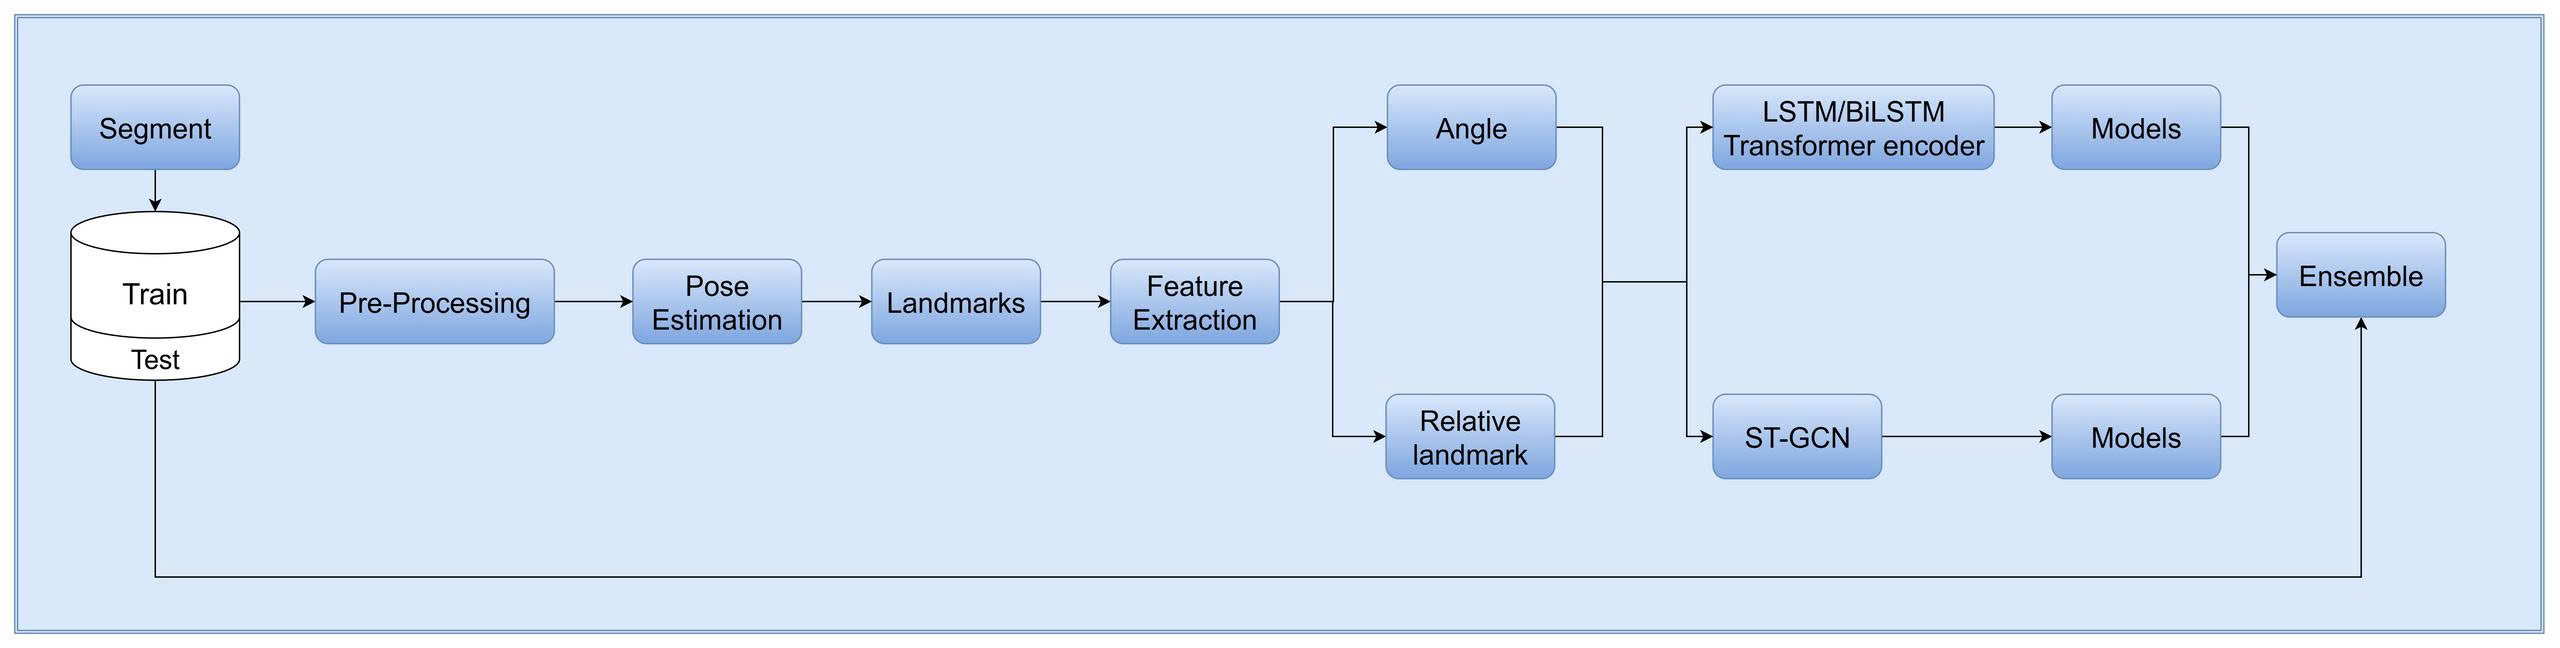
\includegraphics{./images/Pipeline.jpg}}
        \resizebox{0.98\textwidth}{!}{\begin{tikzpicture}[
% Control the style of the blocks
%     node distance=1cm and 0.8cm,
%     base/.style={draw, fill=blue!20, text centered, minimum height=3em, rounded corners=3pt, font=\sffamily\small},
%     block/.style={base, text width=7em},
%     wideblock/.style={base, text width=9em},
    block/.style={
        draw,
        line width=0.3mm,
%         fill=red!10,
        minimum width=2.5cm,   % Your original width (1 - 0)
        minimum height=2cm,  % Your original height (1.5 - -2.5)
        align=center,
        font = \Large,
%         rotate=-90           % This rotates the whole box and text
    },
        blockfe/.style={
        draw,
        line width=0.3mm,
        fill=red!10,
        minimum width=3cm,   % Your original width (1 - 0)
        minimum height=4cm,  % Your original height (1.5 - -2.5)
        align=center,
        font = \Large,
%         rotate=-90           % This rotates the whole box and text
    },
    dataset/.style={
        draw,
        line width=0.3mm,
        fill=green!10,
        minimum width=4cm,   % Your original width (1 - 0)
%         width = 1cm,
        minimum height=1cm,  % Your original height (1.5 - -2.5)
        align=center,
        font = \Large,
%         rotate=-90           % This rotates the whole box and text
    },
    database/.style={
        draw, 
        cylinder, 
        aspect=0.3, 
        shape border rotate=90, 
        line width=0.3mm,
        minimum width=6em, 
        minimum height=8em, 
        text centered, 
        align=center,
       font = \Large,
    },
    sum/.style={
        draw,
        line width=0.3mm,
        circle,
        minimum size=0.5cm, % Matches your 0.25 radius
        inner sep=0pt,      % Ensures the '+' is perfectly centered
%         font=\small
    },
   model/.style = {
   draw, 
   rectangle, 
    minimum width=3cm, 
    minimum height=2cm, 
    line width = 0.3mm,
    align=center,
     font = \Large,
   },
    line/.style={draw, -Stealth, thick}, % stealth , -latex
    arrow/.style={draw, -Stealth, thick}
]





% \draw [line] (10,0) -- (11,1.5)-- (14,1.5)-- (14.5,1.5);
% \draw [line] (10,-0.5) -- (11,1)-- (14,1)-- (14.5,1);
% \draw [line] (10,-1) -- (11,0.5)-- (14,0.5)-- (14.5,0.5);

% \draw [line] (10,0) -- (11,-1.5)-- (14,-1.5)-- (14.5,-1.5);
% \draw [line] (10,-0.5) -- (11,-2)-- (14,-2)-- (14.5,-2);
% \draw [line] (10,-1) -- (11,-2.5)-- (14,-2.5)-- (14.5,-2.5);

% Nodes
%     \node [block] (segment) {Segment};
    \node [database] (database) at (-1,-0.5) {Video \\ dataset};
    \node [dataset] (training) at (4.5,1) {Training set};
     \node [dataset] (validation) at (4.5,-0.5) {Validation set};
     \node [dataset] (testing) at (4.5,-2) {Testing set};
%     \node [block, right=of data] (preproc) {Pre-Processing};
%     \node [block, right=of preproc] (pose) {Pose Estimation};
%     \node [block, right=of pose] (landmarks) {Landmarks};

\draw [line] (0,-0.5) -- (1,-0.5)-- (1,1)-- (training);
\draw [line]  (1,-0.5)-- (2,-0.5)-- (validation);
\draw [line]  (1,-0.5)-- (1,-2)-- (testing);




  
%   \node [sum] (sum1) at (16.5,-0.5) {+};
%  \draw [arrow] (14.5,1) -- (sum1.west);
%   \draw [arrow] (14.5,-2) -- (sum1.west);
%   
%     \node [sum] (sum2) at (16.5,-2) {+};
%  \draw [arrow] (14.5,0.5) -- (sum2.west);
%   \draw [arrow] (14.5,-2.5) -- (sum2.west);
  
   \node [dataset] (trainingfm) at (13.5,1) {Training set \\ feature maps};
     \node [dataset] (validationfm) at (13.5,-0.5) {Validation set\\ feature maps};
     \node [dataset] (testingfm) at (13.5,-2) {Testing set\\ feature maps};
     
        
\draw [arrow] (training.east) -- (trainingfm);
\draw [line] (validation.east) -- (validationfm);
\draw [line] (testing.east)-- (testingfm);

     
     \node [blockfe, fill opacity=0.9, text opacity=1] (feature) at (9,-0.5) {Feature \\ Extraction};
    
%     \draw [arrow] (sum.east) -- (trainingfm);
%     \draw [arrow] (sum1.east) -- (validationfm);
%     \draw [arrow] (sum2.east) -- (testingfm);
    \node [block] (seg) at (1,5.75) {\Large Segment};
    \node [block] (preproc) at (4.5,5.75) {\Large Preprocessing};
     \node [block] (pose) at (8.5,5.75) {\Large Mediapie-based \\ \Large pose landmark \\ \Large estimation};
%      \node [block] (landm) at (8.5,-6) {Landmark \\ extraction};
      \node [block, fill=cyan!10, fill opacity=0.9, text opacity=1] (angle) at (12.5,7.25) {\Large Angle \\ \Large Extraction};
    \node [block, fill=yellow!10, fill opacity=0.9, text opacity=1] (rel) at (12.5,4.25) {\Large Relative \\ \Large Landmark \\ \Large Extraction};
%       \node [sum] (sum) at (14,-6) {+};
      
       \draw [arrow] (-1,5.75) -- (seg) ;
        \draw [arrow] (seg) -- (preproc) ;
     \draw [arrow] (preproc.east) -- (pose) ;
%        \draw [arrow] (pose.east) -- (landm) ;
       \draw [arrow] (pose) -- (10.75,5.75)  -- (10.75,7.25)-- (angle);
       \draw [arrow] (10.75,5.75)  -- (10.75,4.25)-- (rel);
    
   
%  \draw [arrow] (angle)--(14,-5) -- (sum.north);
%   \draw [arrow] (rel)--(14,-7) -- (sum.south);
%     \draw [arrow] (sum)--(15,-6) ;
    
    \draw[dashed, line width = 0.3mm, red](-0.75,3) rectangle(16,8.5);
    
    \draw[ cyan!10,  fill = cyan!10 , line width = 0.3mm](15,5.75) rectangle(15.5,7.5);
    \draw[  yellow!10, fill = yellow!10 , line width = 0.3mm](15,4) rectangle(15.5,5.75);
     \draw[ black , line width = 0.3mm](15,4) rectangle(15.5,7.5);
     \draw[dashed](15,5.75)--(15.5,5.75);
    
    \draw [arrow] (angle)  -- (15,7.25);
    \draw [arrow] (rel)  -- (15,4.25);
    \draw [arrow] (15.5,5.75)  -- (16.25,5.75);
    
    \draw[dashed](-0.75,3)--(7.5,1.5);
      \draw[dashed](16,3)--(10.5,1.5);

\node[align = center, red] at (4.75,9) {\Large proposed feature extraction method for each frame};
\node[align = center] at (14.75,9) {\Large feature map};
\node[align = center, rotate = -90] at (14.75,5.75) {\Large concatenate};
 \draw[arrow, dashed](15.25,8.75)--(15.25,7.75);
 
 \node[model] (model) at (18,-0.5) {LSTM/ \\ BiLSTM/ \\ Transformer};
 \draw[arrow] (trainingfm) --(18,1)-- (model);
  \draw[arrow] (validationfm) -- (model);
  
  \node[model, red] (bestm) at (13.5,-4.75) {Best models};
   \draw[arrow] (model) --(18,-4.75)-- (bestm);
   \draw[arrow] (testingfm) -- (bestm);
   
   \draw[line width = 0.5mm] (8.75,-4.75) ellipse (1.5cm and 0.75cm);
\node[align = center] at (8.75,-4.75) {\Large Evaluations};
 \draw[arrow] (bestm) --(10.25,-4.75);
 
 \node[align = center] at (16.75,1.25) {\Large training};
  \node[align = center] at (14.5,-3.25) {\Large testing};
 
\end{tikzpicture}}
        \caption{The proposed method of feature extraction in the pipeline of training the DL models.}
    \end{center}
    \label{fig:propFs}
\end{figure}

Each raw video is manually trimmed to isolate only the target exercise, producing clean segments. We then generate clips from each segment using a 32-frame sliding window with a 16-frame stride (50\% overlap) for the training set to encourage dense temporal feature representation, while using non-overlapping 32-frame clips (stride of 32 frames) for validation and testing to strictly prevent redundant boundary predictions, padding any final clip by duplicating its last frame to reach 32 frames. This exact procedure is applied to both of our model inputs - the pose-landmark stream and the spatio-temporal graph stream—so that each branch processes input sequences of identical length.


\textbf{MediaPipe} detects 33 landmarks on the human body, each represented by three-dimensional coordinates (x, y, z) and a visibility score indicating the likelihood of the landmark being visible. These landmarks cover major body parts such as shoulders, elbows, wrists, hips, knees, and ankles. In addition to normalized coordinates, MediaPipe provides world landmarks in real-world space, enhancing applications requiring spatial accuracy.	\cite{chuankun2019}

\begin{figure}[!h]
    \centering
    \subfloat[Pose Detection - Hammer Curl]{%
        % \resizebox{0.95\linewidth}{!}{\input{./images/training_ViT.tex}}
        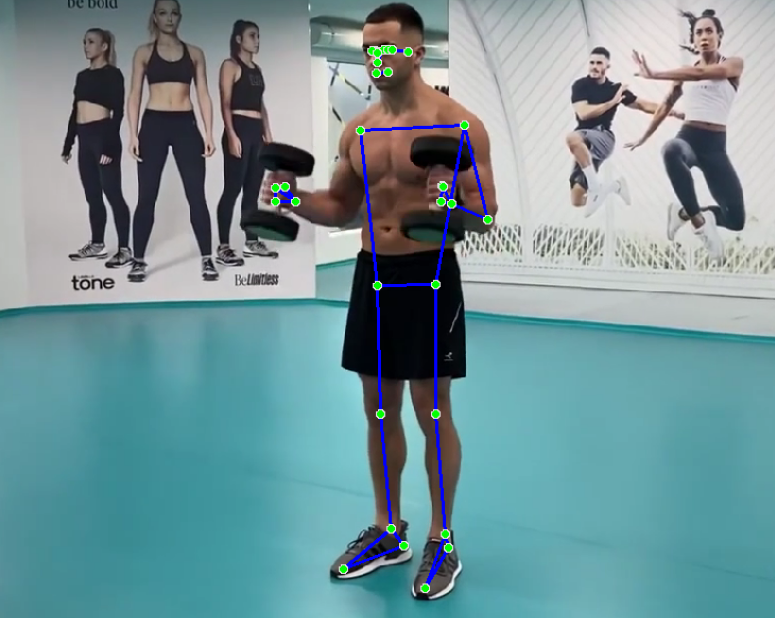
\includegraphics[width=0.45\textwidth]{./images/Mediapipe.png}
        \label{fig:hammer}
    }\hspace{5pt}
\subfloat[Pose Detection - Barbell Biceps Curl]{%
        % \resizebox{0.95\linewidth}{!}{\input{./images/training_ViT_acc.tex}}
        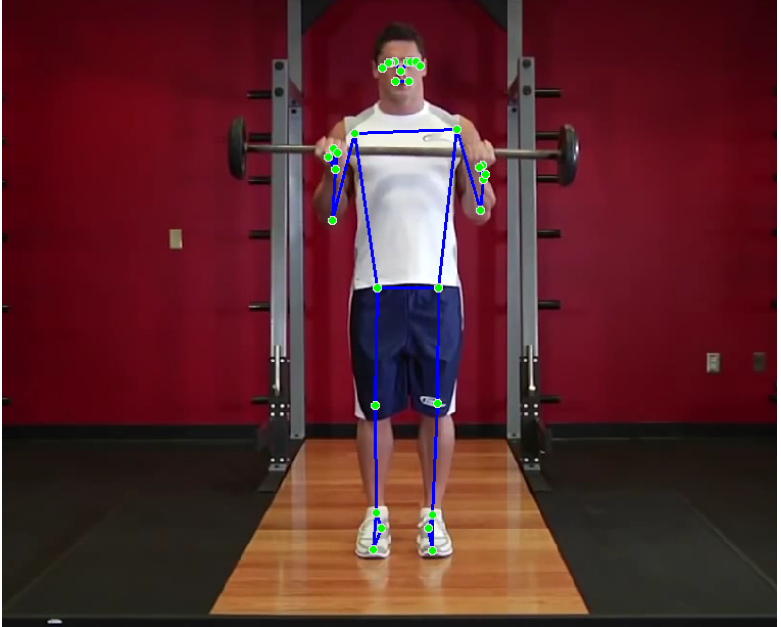
\includegraphics[width=0.45\textwidth]{./images/Mediapipe 2.png}
        \label{fig:barbell}
    }
    \caption{Pose landmark detection results on different frames using MediaPipe.}
    \label{fig:pose_comparison}
\end{figure}

% \begin{figure}[!h]
%     % \hspace*{-1.5cm} % <-- Đẩy ảnh qua bên trái
%     \begin{center}
%         % 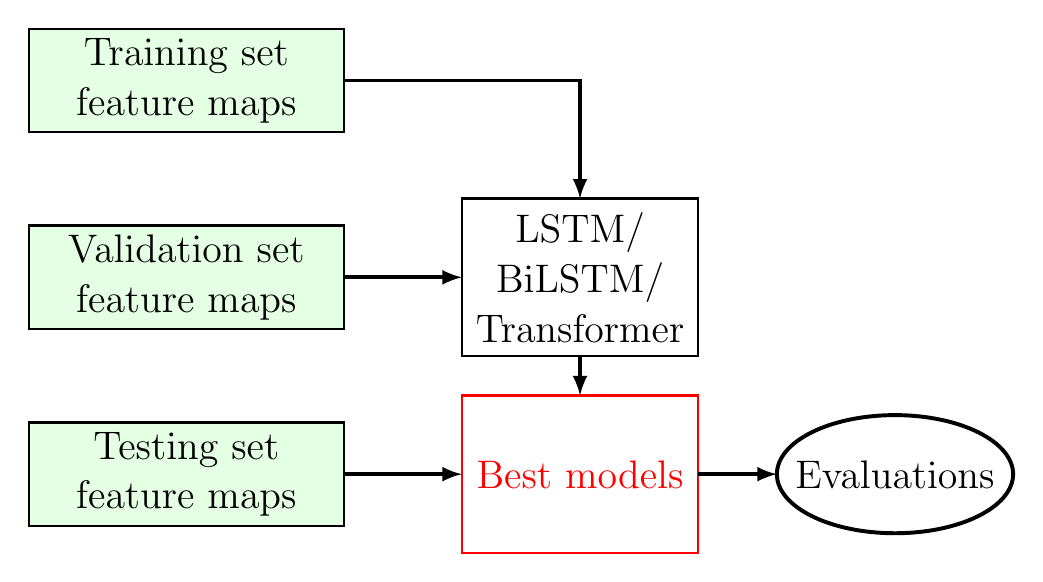
\begin{tikzpicture}[
dataset/.style={
        draw,
        line width=0.3mm,
        fill=green!10,
        minimum width=4cm,   % Your original width (1 - 0)
%         width = 1cm,
        minimum height=1cm,  % Your original height (1.5 - -2.5)
        align=center,
        font = \Large,
%         rotate=-90           % This rotates the whole box and text
    },
   model/.style = {
   draw, 
   rectangle, 
    minimum width=3cm, 
    minimum height=2cm, 
    line width = 0.3mm,
    align=center,
     font = \Large,
   },
 ]

   \node [dataset] (trainingfm) at (3,3.5) {Training set \\ feature maps};
     \node [dataset] (validationfm) at (3,1) {Validation set\\ feature maps};
     \node [dataset] (testingfm) at (3,-1.5) {Testing set\\ feature maps};

\node[model] (bestm) at (8,1) {LSTM/ \\ BiLSTM/ \\ Transformer};
% \draw[line width = 0.5mm] (6.5,0.5) rectangle (9.5,2.5) node[pos = .5, align = center] {DL model};
\draw[line width = 0.5mm, -latex] (5,1) -- (6.5,1);
\draw[line width = 0.5mm, -latex] (5,3.5) -- (8,3.5)-- (8,2);

\node[model, red] (bestm) at (8,-1.5) {Best models};
% \draw[line width = 0.5mm, red] (6.5,-2.5) rectangle (9.5,-0.5) node[pos = .5, align = center, black] {Best model};
\draw[line width = 0.5mm, -latex] (5,-1.5) -- (6.5,-1.5);
\draw[line width = 0.5mm, -latex] (8,0) -- (8,-0.5);
\draw[line width = 0.5mm, -latex] (9.5,-1.5) -- (10.5,-1.5);
\draw[line width = 0.5mm] (12,-1.5) ellipse (1.5cm and 0.75cm);
\node[align = center] at (12,-1.5) {\Large Evaluations};
% \node[align = center] at (2,3.5) {60\%};
% \node[align = center] at (2.5,1.75) {20\%};
% \node[align = center] at (2,-1) {20\%};
\end{tikzpicture}
%         \resizebox{0.7\textwidth}{!}{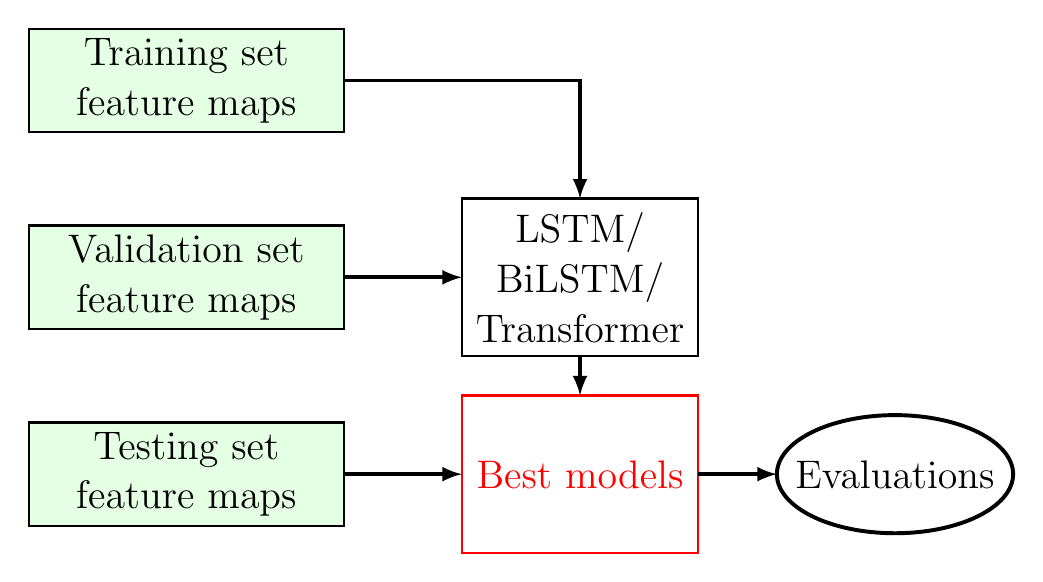
\begin{tikzpicture}[
dataset/.style={
        draw,
        line width=0.3mm,
        fill=green!10,
        minimum width=4cm,   % Your original width (1 - 0)
%         width = 1cm,
        minimum height=1cm,  % Your original height (1.5 - -2.5)
        align=center,
        font = \Large,
%         rotate=-90           % This rotates the whole box and text
    },
   model/.style = {
   draw, 
   rectangle, 
    minimum width=3cm, 
    minimum height=2cm, 
    line width = 0.3mm,
    align=center,
     font = \Large,
   },
 ]

   \node [dataset] (trainingfm) at (3,3.5) {Training set \\ feature maps};
     \node [dataset] (validationfm) at (3,1) {Validation set\\ feature maps};
     \node [dataset] (testingfm) at (3,-1.5) {Testing set\\ feature maps};

\node[model] (bestm) at (8,1) {LSTM/ \\ BiLSTM/ \\ Transformer};
% \draw[line width = 0.5mm] (6.5,0.5) rectangle (9.5,2.5) node[pos = .5, align = center] {DL model};
\draw[line width = 0.5mm, -latex] (5,1) -- (6.5,1);
\draw[line width = 0.5mm, -latex] (5,3.5) -- (8,3.5)-- (8,2);

\node[model, red] (bestm) at (8,-1.5) {Best models};
% \draw[line width = 0.5mm, red] (6.5,-2.5) rectangle (9.5,-0.5) node[pos = .5, align = center, black] {Best model};
\draw[line width = 0.5mm, -latex] (5,-1.5) -- (6.5,-1.5);
\draw[line width = 0.5mm, -latex] (8,0) -- (8,-0.5);
\draw[line width = 0.5mm, -latex] (9.5,-1.5) -- (10.5,-1.5);
\draw[line width = 0.5mm] (12,-1.5) ellipse (1.5cm and 0.75cm);
\node[align = center] at (12,-1.5) {\Large Evaluations};
% \node[align = center] at (2,3.5) {60\%};
% \node[align = center] at (2.5,1.75) {20\%};
% \node[align = center] at (2,-1) {20\%};
\end{tikzpicture}}
%         \caption{The pipeline to train the models.}
%     \end{center}
%     \label{fig:propFs}
% \end{figure}

For the pose‐based branch, each clean video segment was first decomposed into 32-frame clips (using a stride of 16 frames on training segments, and a non-overlapping stride of 32 frames on validation and testing segments), yielding 17\,100 clips (12\,419 training, 2\,228 validation, 2\,453 testing). 
We then applied two complementary feature‐extraction pipelines. In the landmark stream, MediaPipe detects 33 two‐dimensional landmarks per frame, each represented as a 4-dimensional vector $(x, y, z, \text{visibility})$. To focus on the most informative joints, we discard non-essential points (e.g., fingers and toes), retaining 13 key landmarks. From the full 33-landmark set we compute 32 relative-landmark features—inter-joint offsets normalized about the nose—and from the reduced 13-landmark set a further 12 relative features. 
We also compute geometric angles from every triplet of these 13 landmarks ($\binom{13}{3}$ angles total), yielding a compact yet expressive representation.

% In the pose‐based branch, we explore a rich set of spatial features derived from MediaPipe’s 33 4-dimensional landmarks (x, y, z, visibility) per frame, as well as reduced and relative representations for improved robustness. 
First, the raw‐landmark tensor (RawF) comprises all 33 points, each with four values, yielding a (33$\times$4) 132-dimensional feature vector per frame.
\begin{equation}
    l_{RawF} = 33 \times 4 = 132.
\end{equation}

To emphasize head‐centered coordinates, we re-center each frame on the nose landmark and discard its x, y, z values while preserving its visibility score, producing a relative‐raw tensor (RelF) of 129 features per frame.
\begin{equation}
    l_{RelF} = (33 - 1)\times4 + 1 = 129.
\end{equation}

Next, we select 13 semantically important joints (e.g. shoulders, hips, knees), each with four values, to form a key‐landmark tensor of (13$\times$4) 52 features; re-centering these 13 points on the nose and dropping its spatial coordinates (but keeping its visibility) yields a relative‐key tensor of ((13 - 1)$\times$4 + 1) 49 features per frame. Finally, we compute joint angles for every triplet of the 13 key landmarks, resulting in 286 angular features (AngF).
\begin{equation}
    l_{AngF} = \dbinom{13}{3} = 286.
\end{equation}

To evaluate the contribution of each modality, we perform ablation by selectively omitting the $z$ coordinate or the visibility score, resulting in multiple feature variants. 
Each variant—raw 4D landmarks, reduced 13-landmark coordinates, relative offsets, and angle features—is independently modeled by a compact Transformer encoder. 
In parallel, we construct a spatio-temporal graph from the same 13 landmarks and process it through an ST-GCN. 
By systematically studying all feature combinations across both the Transformer and the graph-convolutional models, we assess how each representation contributes to robust, viewpoint-invariant exercise classification.

\subsection{DL models for exercise classification}

After feature maps are extracted, they are fed to the deep learning models to classify the exercises.
Because the feature maps are from consecutive frames, Long Short-Term Memory (LSTM), Bidirectional LSTM (BiLSTM) and Transformer Encoder are selected to process the feature maps of the frame sequence.

\begin{itemize}
    
\item  \textbf{Long Short-Term Memory (LSTM)} networks are employed to model the temporal evolution of exercises. LSTM processes sequences of extracted features to predict the corresponding exercise category. By maintaining memory over long sequences, LSTM effectively captures the progression of movements across time, which is critical for distinguishing between different exercise types.	\cite{hochreiter1997long}

\item \textbf{Bidirectional LSTM (BiLSTM)} networks are introduced to enhance temporal context modeling. BiLSTM simultaneously processes input sequences in both forward and backward directions, allowing the model to incorporate information from both past and future frames. This bidirectional architecture leads to improved understanding of movement patterns and transitions, enhancing classification accuracy.	\cite{graves2005}

\item \textbf{Transformer Encoder} is employed as one of the temporal modeling backbones in the pose-based stream to capture long-range dependencies and complex spatio-temporal relationships between joints. Unlike RNN-based models, which process input sequentially, the Transformer leverages multi-head self-attention to enable direct interactions across all frames in a 32-frame clip, allowing it to attend to motion cues distributed arbitrarily over time. We use a lightweight Transformer encoder with 4 layers and 8 attention heads, followed by a global average pooling and classification head. This architecture is applied to three types of input features: (1) relative landmark coordinates, (2) angular features derived from joint triplets, and (3) the concatenation of both, where we first encode the two modalities separately before fusing their latent representations through an additional Transformer layer. Empirical results show that the Transformer encoder consistently outperforms LSTM and Bi-LSTM baselines across all input types, particularly in the concatenated configuration, where it achieves the highest validation accuracy in the pose stream \cite{plizzari2021sttr}.

\item \textbf{ST‐GCN} is employed as a graph‐based alternative for our pose stream modeling, replacing sequential architectures like LSTM, Bi‐LSTM, and Transformers. Rather than flattening keypoints into vectors, ST‐GCN represents the human body as a structured graph: here we use the 32 relative landmarks (each with x, y, z, and visibility), so each frame yields 32 nodes. Edges connect anatomically adjacent joints within a frame (spatial) - for example, nose-eck, neck-shoulder, shoulder-elbow, elbow-wrist, hip-knee, knee-ankle, etc. - and link each joint to itself in the next frame (temporal). For each 32‐frame window, we assemble a spatio‐temporal graph tensor of shape $(C, T, V) = (2, 32, 32)$, where $C=2$ (the x and y coordinates), $T=32$ frames, and $V=32$ joints. Graph convolutions operate simultaneously over space and time, enabling the model to learn local joint dependencies and dynamic motion patterns directly from the relative landmark inputs. Trained independently with cross-entropy loss, ST‐GCN outperforms our RNN‐based variants, demonstrating superior capacity to recognize spatially complex and temporally extended exercise movements \cite{yan2018stgcn}. 

\end{itemize}

\subsection{Ensemble strategy}


\textbf{Ensemble Strategy} is employed to integrate predictions from multiple temporal and graph-based models across diverse skeletal and angular representations. After independently training all variants, we select the best-performing models based on validation loss. We explore three ensemble methods: (1) \textit{hard voting}, where the final class is determined by majority vote from individual model predictions; (2) \textit{soft voting}, which averages softmax probabilities from the selected models to produce a final prediction; and (3) \textit{stacking}, in which outputs from base models are used as input features to a lightweight meta-classifier trained to make the final decision. Among these, stacking yields the highest overall accuracy, effectively leveraging complementary cues—sequence-based motion dynamics from Transformers/LSTMs and spatial graph relationships from ST-GCN. Overall, ensemble methods consistently outperform single-stream models, highlighting the benefit of multi-model fusion in gym exercise recognition.\cite{wolpert1992stacking}

\subsection{Hyperparameters and Metrics}

\textbf{Evaluation} is based on multiple metrics, including Accuracy, Precision, Recall, and F1-score, to provide a comprehensive assessment of model effectiveness. A confusion matrix is constructed to analyze misclassifications and to identify common sources of errors among exercise classes.

For both the pose‐based and graph‐based branches, we used identical training hyperparameters: up to 100 epochs, early stopping with a patience of 20 epochs on validation loss, a batch size of 16, sequence lengths fixed at 32 frames, with a stride of 16 frames for training and a stride of 32 frames for validation and testing. In the pose stream, each clip’s landmarks and angle are modeled by three temporal architectures - LSTM, Bi‐LSTM, and a Transformer encoder - while in the graph stream the same these landmarks are structured into a spatio-temporal graph and processed by an ST-GCN. All four models were trained and validated under these consistent conditions to enable a fair comparison of their capacity to capture both temporal dependencies and spatial relationships in gym exercise data.

\section{Result and Discussion}

To capture complementary information, we experiment with three input configurations: (a) relative‐keylandmark coordinates alone, (b) angular features alone, and (c) the concatenation of both relative coordinates and angles into a unified 335-dimensional vector (49 + 286). Each clip (32 frames × feature‐dim) is passed through one of three temporal models - LSTM, Bi-LSTM, or a 4-layer, 8-head Transformer encoder - to learn spatio-temporal patterns. In the concatenated variant, we first process relative‐coordinates and angles through separate temporal streams, then fuse their outputs via concatenation followed by an additional Transformer layer to integrate both geometric and kinematic cues. All models are trained independently, and the best‐performing variant on the validation set is selected for the final evaluation.

\begin{table}[!h]
\centering
\caption{Test accuracy (\%) of temporal models on different landmark feature sets}
\label{tab:accuracy-spatial-models}
\begin{tabular}{l c c c c c}
\hline
\textbf{Model}      & \makecell{\textbf{Raw}\\ 33$\times$4} & \makecell{\textbf{Rel.} \\ 32$\times$4+1} & \makecell{\textbf{Raw} \\ 13$\times$4} & \makecell{\textbf{Rel.}\\ 12$\times$4+1} & \textbf{Angle} \\
\hline
LSTM                & 0.2837                   & 0.4339                      & 0.2858                   & 0.4336                      & 0.3987        \\
Bi‐LSTM             & 0.3549                   & 0.4932                      & 0.3344                   & 0.4867                      & 0.4637        \\
Transformer (4×8)   & 0.5185                   & 0.5541                      & 0.5089                   & 0.5185                      & 0.5222        \\
\hline
\end{tabular}
\end{table}

Overall, we observe a clear hierarchy in model performance across all four feature sets: the Transformer outperforms the Bi‐LSTM, and the Bi‐LSTM outperforms the LSTM. While both LSTM and Bi-LSTM struggle with the high-dimensional raw inputs—dropping to approximately 28.37\% and 35.49\% accuracy respectively on the Raw 33×4 dataset—they show significant improvement when using relative coordinates. For example, on the Rel. 32×4+1 feature set, LSTM accuracy reaches 43.39\% and Bi-LSTM 49.32\%, whereas the Transformer climbs to 55.41\%. This suggests that while recurrent architectures benefit greatly from the normalized structure of relative landmarks, the Transformer’s self-attention mechanism is still superior at modeling the intricate spatial relationships, enabling it to achieve over 55\% test accuracy on the most complex feature configuration.

When using the Angle feature set alone—comprising geometric angles from triplets of key joints—the LSTM accuracy reaches 39.87\% and the Bi‐LSTM 46.37\%, demonstrating that relational geometry carries significant discriminative power compared to raw coordinates for recurrent models. The Transformer again leads with 52.22\%, maintaining high performance. These results confirm that while relational angle features are highly informative, the Transformer excels at integrating both spatial magnitudes and relational structures to consistently deliver the highest classification accuracy across different input types.

\begin{table}[!h]
\centering
\caption{Test accuracy (\%) of Transformer on relative 12$\times$4+1 landmarks with different augmentations}
\label{tab:augmentation-results}
\begin{tabular}{l c}
\hline
\textbf{Augmentation Method} & \textbf{Accuracy (\%)} \\
\hline
Jitter                       & 0.5133                 \\
Rotate                       & 0.5404                \\
Joint\_Dropout          & 0.4555                 \\
Time\_Warp                & 0.5113                 \\
\hline
\end{tabular}
\end{table}

All four augmentation techniques were applied to the Transformer trained on the relative 12$\times$4+1 landmark inputs. Contrary to the initial hypothesis, both Jitter (51.33\%) and Time-Warp (51.13\%) failed to improve test accuracy over the unaugmented baseline of 51.85\%. Similarly, Joint-Dropout significantly reduced performance, dropping accuracy to 45.55\%. Crucially, only Rotate achieved a clear uplift - raising accuracy from 51.85\% to 54.04\% - demonstrating that modeling rotational invariance is more effective for this specific feature set than temporal warping or noise injection.

\begin{table}[!h]
\centering
\caption{Test accuracy (\%) of concatenated feature methods on relative 12$\times$4+1 landmarks and angle features}
\label{tab:concat-results}
\begin{tabular}{l c c}
\hline
\textbf{Model}    & \textbf{Branch‐Concat} & \textbf{Direct‐Concat} \\
\hline
LSTM              & 0.4887                 & 0.4086                 \\
Bi‐LSTM           & 0.5075                 & 0.4781                 \\
Transformer   & 0.5684                 & 0.5212                 \\
\hline
\end{tabular}
\end{table}

We evaluated two strategies for fusing relative‐landmark and angle feature streams: direct concatenation of feature vectors prior to temporal modeling, and a branch‐concat approach in which each feature type is first processed by a dedicated temporal sub‐network and their resulting embeddings are then concatenated and integrated. The branch‐concat fusion consistently yields higher test accuracy across all three architectures, indicating its superior capacity to preserve and combine complementary information. Specifically, the Transformer encoder’s accuracy increases from 52.12\% under direct concatenation to 56.84\% with branch‐concat, a gain of 4.72 points. Similarly, the Bi‐LSTM and LSTM models benefit by 2.94 and 8.01 points, respectively. These findings suggest that allowing each feature stream to learn specialized representations before fusion produces richer embeddings, whereas direct concatenation tends to overwhelm a single temporal model with heterogeneous signal types, hindering its ability to disentangle geometric and angular cues

\begin{table}[!h]
\centering
\caption{Test accuracy (\%) of ST‐GCN on raw vs.\ relative landmark inputs}
\label{tab:stgcn-results}
\begin{tabular}{l c c}
\hline
\textbf{Input Type} & \textbf{Raw 33$\times$4} & \textbf{Rel. 32$\times$4+1} \\
\hline
ST‐GCN              & 0.5116                   & 0.4490                     \\
\hline
\end{tabular}
\end{table}

When applied to the full 33-landmark raw input, ST-GCN achieves 51.16\% accuracy. However, when using the 32 relative landmarks (dropping the nose’s spatial coordinates but retaining its visibility), performance drops to 44.90\%, a decrease of 6.26 percentage points. This result indicates that in this specific case, switching to relative representations does not yield the expected improvement. It is possible that the absolute coordinates in the raw data contain critical global spatial information that the relative normalization process inadvertently discarded, making it more difficult for the ST-GCN to learn underlying kinematic features. Consequently, the raw data provides a stronger foundation for human pose classification in this experiment.

\begin{table}[!h]
\centering
\caption{Ensemble performance on the test set using heterogeneous cross-paradigm architectures}
\label{tab:ensemble-results}
\begin{tabular}{l c c c c}
\hline
\textbf{Ensemble Strategy} & \textbf{Component Models} & \textbf{Window Acc (\%)} & \textbf{Macro F1} & \textbf{Video Acc (\%)} \\
\hline
Hard Voting (T5.1)                  & Transformer + AAGCN Joint & 54.26 & 0.5884 & -- \\
Soft Voting (T5.2)                  & Transformer + AAGCN Joint & 61.46 & 0.6347 & -- \\
Stacking Meta-Learner (T5.3)        & Transformer + AAGCN Joint & \textbf{62.21} & \textbf{0.6367} & -- \\
Tri-Model Grand Ensemble (T5.4)     & Transformer + AAGCN Joint + Bone & 60.25 & 0.6341 & 77.54 \\
Grand 5-Stream SOTA Ensemble (T5.5) & Transformer + 4-Stream AAGCN & 60.22 & 0.6353 & \textbf{78.39} \\
\hline
\end{tabular}
\end{table}

We ensemble the strongest individual models across paradigms—the self-attention Transformer ($M_{seq}^*$ trained on 3D coordinates with dynamic SkelGym-Aug) and the spatial-temporal graph models ($M_{graph}^*$, including Adaptive Graph Convolutional Networks across joint, bone, and motion modalities). Both voting schemes significantly improve upon individual baselines, with soft voting achieving 61.46\% and stacking meta-learning yielding the highest window-level accuracy at 62.21\% (Macro F1 = 0.6367). Crucially, extending the ensemble across four adaptive graph streams (joint, bone, joint-motion, bone-motion) and applying temporal consensus aggregation across full video clips elevates classification performance to 78.39\% accuracy and a 0.7951 Macro F1 score on the held-out test videos.

\begin{table}[!h]
\centering
\caption{Detailed classification report for the Grand SOTA ensemble across all 22 gym exercise classes}
\label{tab:stacking-report}
\begin{tabular}{l c c c r}
\hline
\textbf{Exercise Class}   & \textbf{Precision} & \textbf{Recall} & \textbf{F1-score} & \textbf{Support} \\
\hline
barbell biceps curl       & 0.2646             & 0.7246          & 0.3876            & 69               \\
bench press               & 0.2995             & 0.6633          & 0.4127            & 98               \\
chest fly machine         & 0.7297             & 0.9878          & 0.8394            & 82               \\
deadlift                  & 0.3194             & 0.6866          & 0.4360            & 67               \\
decline bench press       & 0.2286             & 0.5156          & 0.3168            & 192              \\
hammer curl               & 0.3148             & 0.3018          & 0.3082            & 169              \\
hip thrust                & 0.8086             & 0.3201          & 0.4586            & 528              \\
incline bench press       & 0.8654             & 0.5696          & 0.6870            & 79               \\
lat pulldown              & 0.6048             & 0.9619          & 0.7426            & 105              \\
lateral raise             & 0.9714             & 0.8500          & 0.9067            & 160              \\
leg extension             & 0.7194             & 0.9792          & 0.8294            & 144              \\
leg raises                & 0.9792             & 0.4052          & 0.5732            & 116              \\
plank                     & 0.9250             & 0.6607          & 0.7708            & 56               \\
pull Up                   & 0.7264             & 0.8750          & 0.7938            & 88               \\
push-up                   & 0.7965             & 0.9890          & 0.8824            & 91               \\
romanian deadlift         & 0.6466             & 0.5181          & 0.5753            & 166              \\
russian twist             & 0.8784             & 0.8725          & 0.8754            & 149              \\
shoulder press            & 0.7387             & 0.3727          & 0.4955            & 220              \\
squat                     & 0.8386             & 0.7305          & 0.7808            & 256              \\
t bar row                 & 0.5447             & 0.5194          & 0.5317            & 129              \\
tricep Pushdown           & 0.6931             & 0.7527          & 0.7216            & 93               \\
tricep dips               & 0.7713             & 0.5622          & 0.6504            & 402              \\
\hline
\multicolumn{1}{l}{\textbf{Accuracy (Window)}} &          &                 & \textbf{0.6022}   & 3459             \\
\multicolumn{1}{l}{\textbf{Macro avg}}         & 0.6666   & 0.6736          & \textbf{0.6353}   & 3459             \\
\multicolumn{1}{l}{\textbf{Weighted avg}}      & 0.6955   & 0.6022          & 0.6097            & 3459             \\
\hline
\multicolumn{1}{l}{\textbf{Video Consensus Acc}} &        &                 & \textbf{0.7839}   & 236 videos       \\
\multicolumn{1}{l}{\textbf{Video Macro F1}}    & 0.8353   & 0.7941          & \textbf{0.7951}   & 236 videos       \\
\hline
\end{tabular}
\end{table}

\begin{figure}[!h]
    % \hspace*{-1.5cm} % <-- Đẩy ảnh qua bên trái
    \begin{center}
        
\includegraphics[width=0.98\textwidth]{./images/confusion_matrix_stacking.png}
        % \resizebox{0.7\textwidth}{!}{
\includegraphics{./images/confusion_matrix_stacking.png}}
        \caption{Confusion matrix of the ensemble model on the test set}
        \label{fig:confmatr}
    \end{center}
\end{figure}

The stacking ensemble achieves an overall window accuracy of 62.21\%, while the multi-stream Grand SOTA ensemble attains 60.22\% window accuracy and 78.39\% under video-level temporal consensus aggregation. Class-level metrics reveal that visually distinct and planar-constrained exercises—such as lateral raise (F1 = 0.9067), push-up (F1 = 0.8824), and russian twist (F1 = 0.8754)—are recognized with high reliability. In video-level evaluation, several classes achieve 100\% precision and recall, effectively overcoming single-frame transitional noise.

Conversely, classes with subtle biomechanical differences or similar postural planes, such as decline bench press (F1 = 0.3168) and hammer curl (F1 = 0.3082), remain challenging. The macro-average F1-score (0.6353 window, 0.7951 video) underscores that performance gains are distributed robustly across both frequent and rare exercise categories.

\section{Conclusion \& Future Work}

In this study, an end-to-end framework integrating 3D MediaPipe pose landmarks, kinematic coordinate representations, spatial-temporal graph modeling, and cross-paradigm ensembling was presented for gym exercise classification. Experiments demonstrate that relative coordinate normalization and dynamic skeletal augmentation (SkelGym-Aug) substantially outperform unaugmented baselines, producing consistent accuracy boosts across sequence transformers (+4.83\% to 57.59\%), ST-GCN (+8.67\%), and adaptive graph networks (+3.18\%). By fusing complementary sequence representations and multi-stream adaptive graph convolutions via stacking and temporal consensus aggregation, the proposed architecture achieves 62.21\% window accuracy and reaches 78.39\% accuracy (0.7951 Macro F1) across 22 common gym exercises on complete held-out test videos.

In future work, we will extend this research by exploring multimodal sensor fusion, applying focal loss and advanced class weighting to further mitigate sample imbalance, investigating self-supervised pretraining on larger skeleton archives, and deploying real-time form correction feedback for smart home fitness systems.

%
% ---- Bibliography ----
%
% BibTeX users should specify bibliography style 'splncs04'.
% References will then be sorted and formatted in the correct style.
%
% \bibliographystyle{splncs04}
% \bibliography{mybibliography}
%
\begin{thebibliography}{100}
\bibitem{donahue2015}
Donahue, J., Hendricks, L. A., Guadarrama, S., Rohrbach, M., Venugopalan, S., Saenko, K., \& Darrell, T. (2015). 
\textit{Long-term recurrent convolutional networks for visual recognition and description}. 
In Proceedings of the IEEE Conference on Computer Vision and Pattern Recognition (CVPR), pp. 2625–2634.
https://arxiv.org/pdf/1411.4389

\bibitem{li2017}
Li, C., Wang, P., Wang, S., Hou, Y., \& Li, W. (2017). 
\textit{Skeleton-based action recognition using LSTM and CNN}. arXiv:1707.02356. 
https://arxiv.org/pdf/1707.02356

\bibitem{yan2018}
Yan, S., Xiong, Y., \& Lin, D. (2018). 
\textit{Spatial Temporal Graph Convolutional Networks for Skeleton-Based Action Recognition}. https://arxiv.org/abs/1801.07455

\bibitem{arnab2021}
Arnab, A., Dehghani, M., Heigold, G., Sun, C., Lučić, M., \& Schmid, C. (2021). 
\textit{ViViT: A Video Vision Transformer}. arXiv:2103.15691. 

\bibitem{riccio2024}
Riccio, R. (2024). \textit{Real-Time Fitness Exercise Classification and Counting from Video Frames}. arXiv preprint arXiv:2411.11548v1.
https://arxiv.org/html/2411.11548v1

\bibitem{abdillah2023}
Abdillah, H. (2023). \textit{WorkoutFitness Video}. Kaggle Dataset. https://www.kaggle.com/datasets/hasyimabdillah/workoutfitness-video

\bibitem{Freepik}
Freepik. Free graphic resources for everyone. From \url{https://www.freepik.com}

\bibitem{Pexels}
Pexels. Free stock photos and videos shared by talented creators. From \url{https://www.pexels.com/}


\bibitem{chuankun2019}
Chuankun, L., Shuang, W., Wanqing, L., Pichao, W., \& Yonghong, H. (2019). 
\textit{MediaPipe: A Framework for Building Perception Pipelines}.
https://arxiv.org/pdf/1906.08172

\bibitem{hochreiter1997long}
Hochreiter, S., \& Schmidhuber, J. (1997). 
\textit{Long Short-Term Memory}. Neural Computation, 9(8), 1735-1780. https://www.bioinf.jku.at/publications/older/2604.pdf

\bibitem{graves2005}
Graves, A., Fernández, S., \& Schmidhuber, J. (2005). 
\textit{Bidirectional LSTM networks for improved phoneme classification and recognition}. In Artificial Neural Networks: Formal Models and Their Applications–ICANN 2005 (pp. 799–804). Springer, Berlin, Heidelberg.
https://www.researchgate.net/publication/221080352

\bibitem{plizzari2021sttr}
Plizzari, C., Cannici, M., \& Matteucci, M. (2021). 
\textit{Skeleton-based Action Recognition via Spatial and Temporal Transformer Networks}. 
Computer Vision and Image Understanding, 208–209, 103219.

\bibitem{ng2015}
Ng, J. Y.-H., Hausknecht, M., Vijayanarasimhan, S., Vinyals, O., Monga, R., \& Toderici, G. (2015). \textit{Beyond short snippets: Deep networks for video classification}.
https://arxiv.org/pdf/1503.08909

\bibitem{szegedy2016}
Szegedy, C., Vanhoucke, V., Ioffe, S., Shlens, J., \& Wojna, Z. (2016).
\textit{Rethinking the Inception Architecture for Computer Vision}.
https://arxiv.org/pdf/1512.00567v3

\bibitem{yan2018stgcn}
Yan, S., Xiong, Y., \& Lin, D. (2018).
\textit{Spatial–Temporal Graph Convolutional Networks for Skeleton-Based Action Recognition}.
https://arxiv.org/abs/1801.07455

\bibitem{ko2024augmentation}
Ko, H., Lee, J., Kim, Y., et al. (2024). 
\textit{Data Augmentation for Efficient Skeleton-Based Action Recognition: Spatial and Temporal Approaches}. 
Electronics, 13(4), 747. 
DOI: \url{https://doi.org/10.3390/electronics13040747}

\bibitem{wolpert1992stacking}
Wolpert, D. H. (1992). \textit{Stacked Generalization}. \emph{Neural Networks}, 5(2), 241–259. https://doi.org/10.1016/S0893-6080(05)80023-1

% \bibitem{liu2021}
% Liu, Z., Ning, J., Cao, Y., Wei, Y., Zhang, Z., Lin, S., \& Hu, H. (2021). 
% \textit{Video Swin Transformer}.
% https://arxiv.org/pdf/2106.13230

% \bibitem{Xi2024}
% Xinyao Xi and Chen Zhang and Wen Jia and Ruxue Jiang (2024). ``\textit{Enhancing human pose estimation in sports training: Integrating spatiotemporal transformer for improved accuracy and real-time performance}. Alexandria Engineering Journal, pp 144-156, vol. 109. DOI: 10.1016/j.aej.2024.08.072

% \bibitem{Mahyoub2024}
% Mohamed Mahyoub, Friska Natalia, Sud Sudirman and Jamila Mustafina, ``\textit{Sign Language Recognition using Deep Learning}'',
% 2023 15th International Conference on Developments in eSystems Engineering (DeSE), Jan. 2023

\end{thebibliography}


\end{document}
